% preambule dokumentu
\documentclass[12pt]{article}
\usepackage[utf8]{inputenc}
\usepackage[czech]{babel}
\usepackage{cite}
\usepackage[pdf]{graphviz}
\usepackage{mathtools}
\usepackage{dipp8, xltxtra, graphicx}
\usepackage{pgfplots}

\begin{document}
\pagestyle{headings}

\def\typprace{Diplomová}

% uvodni cast zaverecne prace
\titul{Řízení autonomního agenta pomocí neuroevoluce}{Bc. Martin Hnátek}{Ing. Jiří Lýsek, Ph.D.}{Brno, 2018}
\podekovani{Rád bych zde poděkoval svému vedoucímu Ing. Jiří Lýskovi, Ph.D. za jeho rady a čas, který mi věnoval při řešení této práce.}
\prohlasenimuz{V Brně dne \today}

\abstract{Autonomous agent control using neuroevolution}{}
% TODO: Lepší abstract
\abstrakt{Řízení autonomního agenta pomocí neuroevoluce}{Tato práce se zabývá trénováním autonomního agenta - auta s pomocí algoritmu neuroevoluce. Toto zahrnuje tvorbu simulačního prostředí pro agenta, vhodným návrhem agenta (senzorů a řízení) a také návrhem fitness funkce}
\obsah
\cislovat{2}

% jednotlive kapitoly dokumentu
\kapitola{Úvod a cíl práce}
\sekce{Úvod do problematiky}
S růstem výpočetního výkonu a rozvojem \textbf{GPUGPU} (paralelizace výpočtů na grafické kartě) se neuronové sítě ukázaly jako mocný nástroj pro řešení složitých problémů na které standardní metody umělé inteligence nestačily.

Další oblastí umělé inteligence, které nárust masivní paralelizace prospěl, jsou metaheuristiky, které mohou  s nárůstem výpočetního výkonu v rozmném čase pokrýt stále větší stavový prostor a jsou tedy schopné rychle řešit stále složitější problémy.


Neuroevoluce propojuje oba přístupy a využívá je ke generování topologii neuronových sítí a nastavení jejích vah. Výsledkem je neuronová síť, jejiž architektura lépe popisuje daný problém a lze jí aplikovat i na problémy na které by klasické neuronové sítě aplikovat nešly. Jedná se například o problémy, u kterých je těžké získat trénovací data a nelze tedy neuronovou síť natrénovat klasickými metodami, jako je například gradientní sestup.

\sekce{Cíl práce}
Cílem této práce je navrhnout a vytvořit simulační prostředí pro autonomního agenta. Poté na simulovaném prostředí provést serii experimentů, které slouží k zjištění limitů učících schopností algoritmu NEAT.

\sekce{Neuronové sítě}

Neuronové sítě jsou model strojového učení, který je volně založený na principu zvířecího mozku \cite[s.~41]{fundementalsOfDeepLearning}.

\sekce{Neuron}
Neuron je základní  výpočetní jednotka neuronových sítí, která je definovaná jako suma všech jejích vstupů a aplikace aktivační funkce.
	$$\sigma(\Sigma_{i=0}^{N} \theta_i \cdot x_{i} + b)$$
Kde:
\begin{enumerate}
	\item $\sigma$ - aktivační funkce
	\item $\theta$ - skrytá váha pro daný vstup
	\item b - bias neuronu
\end{enumerate}

\sekce{Vrstva}
Vrstva je skupina neuronů se stejnou aktivační funkcí. 

\podsekce{Aktivační funkce}
Aktivační funkce se používá pro definování výstupu a zavedení nelinearity. Bez nich by byla neuronová síť schopna aproximovat pouze n-dimenzionální rovinu. \cite[s.~65]{fundementalsOfDeepLearning} \\
Dalším využitím je omezení výstupních hodnot. Například aktivační funkce sigmoid se s oblibou používá u výstupní vrstvy neuronových sítí určených ke klasifikačním problémům, protože je to relace $\mathbb{R} \rightarrow \{0..1\}$, která se dá jednoduše jako "jistota" neuronu, že se jedná o výstup, který neuron reprezentuje. Podobně se dá uvažovat i o funkcích jako je například softmax a tanh, které také najdou hojné využití u klasifikačních problémů.

\podsekce{Linearní funkce}
Vrací vstup, tak jak je. Využití najde především u vstupní vrstvy neuronové sítě a u neuronových sítí, které řeší regresní typy úloh.
\\
\begin{tikzpicture}
\centering
\begin{axis}[grid=major, xlabel=$x$, ylabel={$f(x)$}]
\addplot[blue, samples=100, smooth, unbounded coords=discard]
plot (\x, \x);
\end{axis}
\end{tikzpicture}
$$f(x) = x$$
\podsekce{Sigmoid}
Sigmoid je aktivační funkce, která je schopná potlačit extrémní hodnoty 

\begin{tikzpicture}
\centering
\begin{axis}[grid=major, xlabel=$x$, ylabel={$f(x)$}]
\addplot[blue, samples=100, smooth, unbounded coords=discard]{1 / (1 + e ^ (-\x))};
\end{axis}
\end{tikzpicture}
$$f(x) = \frac{1}{1 + e^{-x}}$$
\podsekce{Tanh}

\textbf{Tanh} je funkce obdobná sigmoidu. Hlavní rozdíl mezi ní a sigmoidem je ten, že její obor je v rozmezí -1 a 1 hodí se proto i pro záporná výstupy, které vyžadují záporná čísla. \cite[s.~67]{fundementalsOfDeepLearning}

\begin{tikzpicture}
\centering
\begin{axis}[grid=major, xlabel=$x$, ylabel={$f(x)$}]
\addplot[blue, samples=100, smooth, unbounded coords=discard]{tanh(x)};
\end{axis}
\end{tikzpicture}
$$f(x) = tanh(x)$$
\podsekce{RELU}
RELU je aktivační funkce, která je podobná lineární aktivační funkci s tím rozdílem, že pokud vstupní hodnota nepřesáhne určitého prahu výstupem je 0. Její hlavní výhodou je to, že zabraňuje problémům s takzvaným explodujícím gradientem \cite[s.~69]{fundementalsOfDeepLearning} \\

\begin{tikzpicture}
\centering
\begin{axis}[grid=major, xlabel=$x$, ylabel={$f(x)$}]
\addplot[blue, samples=100, smooth, unbounded coords=discard]{max(0, x)};
\end{axis}
\end{tikzpicture}
\[ 
f(x) = 
\begin{dcases*} 
\text{$x>=0$,} & $x$ \\ 
\text{$x<0$,} & 0 
\end{dcases*} 
\]
\podsekce{Rekurentní neurony}
Speciální druh neuronů, který si dokáže zapamatovat a reagovat na sekvenci vstupů. Rekurentní neurony značně rozšiřují možnosti neuronových sítí. S nimi je možné řešit složité úlohy typu strojového překladu nebo sémantické vyhodnocování textu.

V praxi se setkáváme s dvěma druhy neuronů a to LSTM a novější GRU. LSTM a GRU jsou si velmi podobné s jedním podstatným rozdílem. U GRU bylo prokázáno, že je značně rychlejší. 


\kapitola{Genetické algoritmy}
Genetické algoritmy slouží k řízenému prohledávání stavového prostoru založené na teorii evoluce. \cite[s.~17]{kozaGP}
\sekce{Princip}
Základní myšlenka spočívá ve vygenerování náhodných jedinců (řešení problému) a jejích postupné zlepšování s pomocí operací křížení a mutace. Proces zlepšování genomů probíhá na základě jeho hodnocení (fitness).

Samotný algoritmus pak lze rozdělit na následující kroky \cite[s.~12]{geneticAlgorithms}

\begin{enumerate}
	\item Vygeneruj náhodnou populaci o n chromozomech
	\item Pro každý chromozom spočítej jeho fitness
	\item Opakuj dokud není splněná podmínka ukončení
	\begin{enumerate}
		\item Vyber pár chromozomů na základě jejích ohodnocení (selekce)
		\item Proveď spojení chromozomů (křížení)
		\item S určitou pravděpodobností mutuj daného jedince (mutace)
	\end{enumerate}
	\item Nahraď současnou populaci populací, která vznikla předchozím krokem
	\item Jdi na krok 2
\end{enumerate}

\sekce{Kódování}
Někdy se mu též říká genotyp je způsob zápisu řešení problému. Je důležité zároveň uvést pojem fenotyp který označuje vlastní řešení úlohy.

Existuje mnoho různých kódování a každý má své výhody a nevýhody. Většinou se snažíme vybírat kódování, které dobře reprezentuje daný problém. Zde je seznam několika nejpoužívanějších kódování \cite[s.~42-43]{geneticCZ}:
\begin{enumerate}
	\item Binární - řetězec bitů, který může například reprezentovat jednu nebo více numerických hodnot. 
	\item Reálná čísla - Jedno nebo více reálných čísel
	\item Kombinatorické - Může být například seznam čísel označujících 
\end{enumerate}
\sekce{Křížení}
Křížení je operátor, který kombinuje dva jedince do jednoho. Jedinec, který vzniká přebírá genetickou informaci od obou jedinců v určitém poměru. Jeho implementace je závislá na použitém kódování. 

Příkladem může být obrázek \ref{fig:crossover} ve kterém je ilustrováno tzv. jednobodové křížení \cite[s.~50]{geneticCZ} při kterém dochází k rozdělení obou genomů ve stejném bodě a spojením vzniklých podřetězců do nového genomu.
	
\begin{figure}[ht]
	\centering
	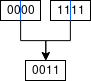
\includegraphics[scale=0.95]{crossover}
	\caption{Příklad křížení}
	\label{fig:crossover}
\end{figure}

\sekce{Mutace}
Mutace náhodně modifikuje chromozom a zavádí tak do populace variaci. Díky tomuto se může algoritmus dostat z lokálního extrému. 

Existují různé varianty mutace, která se provádí v závislosti na daném kódování. 

Například u binárního kódování se může jednat o náhodnou inverzi některého z bitů genomu viz obrázek \ref{fig:mutation}.

\begin{figure}[h!]
	\centering
	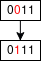
\includegraphics[scale=1.0]{mutation}
	\caption{Příklad mutace}
	\label{fig:mutation}
\end{figure}

\sekce{Selekce}
Selekce je proces výběru dvou jedinců na něž jsou později aplikovány genetické operátory jako je křížení a mutace. 

\sekce{Využití}
Genetické algoritmy naleznou využití v mnoha optimalizačních úlohách. Příkladem může být experiment, který zahrnoval použití gramatické evoluce pro vytvoření regresních modelů pro datasety CASY3 a CASY5 \cite[s.~2-9]{differentialEvolution}.

\kapitola{NEAT}
NEAT (neuroevolution of augmenting topologies) kombinuje neuronové sítě s genetickými algoritmy. Hlavní výhodou této metody je, že generuje jak topologii neuronové sítě, tak její váhy. Výsledkem může být neuronová síť jejíž rozložení lépe popisuje řešený problém.

Algoritmus probíhá stejně jako běžný genetický algoritmus. Rozdílem je použitý fenotyp a operátory mutace a křížení, které se nad ním provádí.

\sekce{Genotyp a fenotyp}
Genotyp a fenotyp je ilustrován na obrázku \ref{fig:neatgenotypetophenotype}. Genotyp obsahuje jak údaje o jednotlivých neuronech, tak informace o topologii sítě. Metadata, která se týkají topologie neuronové síti jsou údaje o spojení (IN, OUT), váha samotného spojení (weight), informace týkající se toho, zda je spojení použito v fenotypu (ENABLED/DISABLED) a inovační skore. Inovační skore je číslo, které reprezentuje pořadí ve kterém se daný gen objevil v fenotypu \cite[s.~9]{NEAT}. 

\begin{figure}[h!]
	\centering
	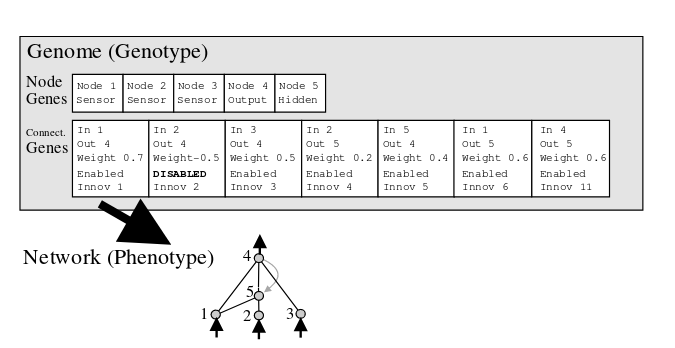
\includegraphics[width=0.7\linewidth]{neatGenotypeToPhenotype}
	\caption{Genotyp a fenotyp u algoritmu NEAT převzato z \cite[s.~9]{NEAT}}
	\label{fig:neatgenotypetophenotype}
\end{figure}

\sekce{Mutace}
Jak jíž bylo zmíněno nad fenotypem lze provádět různé operace včetně operátoru mutace, který provede náhodnou změnu fenotypu s nadějí, že změna povede k zlepšení řešení. V případě algoritmu NEAT je operátor mutace ilustrován na obrázku \ref{fig:neatmutation}. Na obrázku je vidět, že mutace může buď přidat další spojení nebo další neuron. V případě, že je přidávan nový neuron je mu přiřazeno náhodné spojení, které je označeno znakem DISABLED \cite[s.~10]{NEAT}.

\begin{figure}[h!]
	\centering
	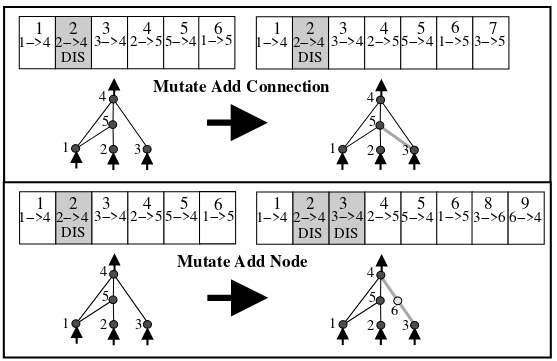
\includegraphics[scale=0.3]{neatMutation}
	\caption{Mutace v NEAT převzato z \cite[s.~10]{NEAT}}
	\label{fig:neatmutation}
\end{figure}

\sekce{Křížení}
Posledním operátorem používaným při algoritmu NEAT je operátor křížení. Operátor křížení ilustruje obrázek \ref{fig:neatcrossover}. Křížení probíhá na základě inovačního čísla. Spojení se stejným inovačním číslem jsou náhodně zděděny z rodičovských genů. Je tu také šance na převzetí genů, které vytváří spojení nenacházející se v jednom z rodičů. Tyto geny jsou převzaty pouze z rodiče, který ma větší fitness. Při křížení je také náhodná šance, která může převzatý genom vypnout \cite[s.~12]{NEAT}.

\begin{figure}[h!]
	\centering
	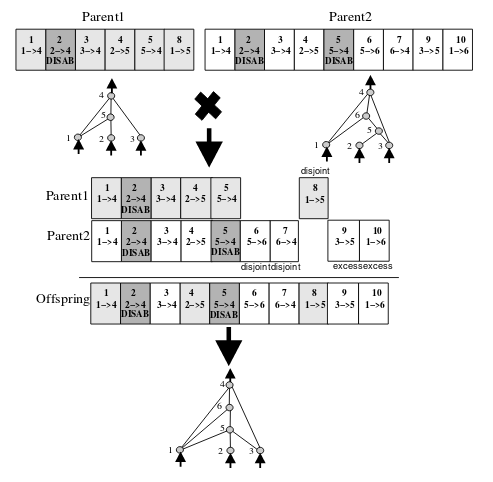
\includegraphics[width=0.6\linewidth]{neatCrossover}
	\caption{Křížení v NEAT. Převzato z \cite[s.~12]{NEAT}}
	\label{fig:neatcrossover}
\end{figure}

\sekce{Rozšíření algoritmu NEAT}
Jelikož je algoritmus NEAT v současnosti předmětem aktivního výzkumu existuje pro něj mnoho rozšíření. Tato sekce se bude zabývat některými z nich.

\podsekce{Instinct}
Instinct rozšiřuje původní algoritmus o rekurentní neurony. Rozšíření tak umožňuje případnému agentovi reagovat nejen na okamžitou situaci ale i na předchozí události ve světě. Tento fakt značně rozšiřuje možnosti neuronových sítí, které jsou generované tímto algoritmem ale zároveň je třeba mít na paměti, že se tímto značně zvětšuje prohledávaný stavový prostor a dochází tím k zvýšené časové náročnosti na získání vhodných výsledků.
\podsekce{odNEAT}
Varianta algoritmu NEAT aplikovaná na distribuované online učení skupiny autonomních robotů \cite[s.~1]{odNEAT}.
\podsekce{rtNEAT}
Rozšíření, které se zaměřuje na neuroevoluci agentů v realném čase.
%In 2003 Stanley devised an extension to NEAT that allows evolution to occur in real time rather than through the iteration of generations as used by most genetic algorithms. The basic idea is to put the population under constant evaluation with a "lifetime" timer on each individual in the population. When a network's timer expires its current fitness measure is examined to see whether it falls near the bottom of the population, and if so it is discarded and replaced by a new network bred from two high-fitness parents. A timer is set for the new network and it is placed in the population to participate in the ongoing evaluations.

%The first application of rtNEAT is a video game called Neuro-Evolving Robotic Operatives, or NERO. In the first phase of the game, individual players deploy robots in a 'sandbox' and train them to some desired tactical doctrine. Once a collection of robots has been trained, a second phase of play allows players to pit their robots in a battle against robots trained by some other player, to see how well their training regimens prepared their robots for battle.

\podsekce{HyperNEAT}
HyperNEAT rozšiřuje neuroevoluci o možnost vytváření velmi velkých neuronových sítí \cite[s.~1]{hyperNEAT}.

\podsekce{cgNEAT}
Rozšíření zaměřující se na generování náhodného obsahu. Obdobně jako tomu je například u GAN sítí.

\sekce{Alternativy k neuroevoluci}
Neuroevoluce není jediný přístup, který je dostupný k řešení problému typu trénování autonomního agenta.

Příkladem může být rozsáhlý obor zabývající se zpětnovazebním učením (reinforcement learning). Při zpětnovazebním učení máme agenta, který se nachází v prostředí nad kterým může vykonávat různé akce. Agent může před vykonáním akce pozorovat stav prostředí na základě čehož se rozhoduje, jakou akci vykoná. Po provedení některé se prostředí nějakým způsobem mění a agent dostává zpětnou vazbu v podobně odměny. Algoritmus zpětnovazebního učení se snaží agenta řídit tak, aby maximalizoval jeho odměnu. 

\kapitola{Použité technologie}
Tato kapitola poskytuje stručný přehled technologii použitých při řešení diplomové práce.

\sekce{Docker}
Docker je nástroj, který umožňuje vytvářet tzv. kontejnery. Kontejner poskytuje izolované softwarové prostředí ve kterém lze spouštět jednu nebo více aplikací. 
V praxi to umožňuje snadné nasazení libovolné aplikace bez ohledu na aktuální konfiguraci hostitelského systému.

\sekce{Vue}
Je populární javascript framework pro snadnou tvorbu uživatelských rozhraní.

\sekce{Node.js}
Node.js je open-source interpret jazyku javascript. Využití najde při psaní serverových aplikací v javascriptu a jiné případy, kdy je třeba spustit kód napsaný v javascriptu mimo prohlížeč. Lze ho využít například pro spouštění testů při CI (continuous integration) nebo pro tvorbu vysoce serverových aplikací v javascriptu.

Narozdíl od běžného javascriptu obsahuje rozšířenou standardní knihovnu pro snadnou tvorbu serverových aplikací. Tato standardní knihovna umožňuje například javascript kódu prácí se soubory na hostitelském systému, což je něco, co není z bezpečnostních důvodů v klasickém javascriptu, který běží v prohlížeči možné.

\sekce{Bull}
Bull je knihovna pro Node.js, která poskytuje frontu úkolů založenou na populární in-memory databázi REDIS.

\sekce{PostgreSQL}
Populární databázový systém, který nabízí robustní open source alternativu i ke komerčním řešením.

\sekce{PIXI.js}
Grafická knihovna pro snadné vykreslování nad html 5 canvasem. Obaluje jak klasické vykreslovací api, tak modernější webgl.

\sekce{Neataptic}
Knihovna implementující samotný algoritmus NEAT ve variantě instinct.

\sekce{NPM a YARN}
NPM i Yarn jsou kolíčkovací systémy pro javascript. Hlavní rozdíl mezi NPM a Yarn je, že Yarn stahuje balíčky paralelně. Je tedy značně rychlejší oproti NPM. 

\sekce{CES}
\label{sec:ces}
Je knihovna, která implementuje tzv. ECS (entity component system). ECS se používá především ve hrách a nabízí určitý způsob, jak se dívat na herní objekty a logiku. Myšlenka je taková, že vše lze rozdělit do níže uvedených podsekcí.

\podsekce{Komponenta}
Komponenty bývají jednoduché datové struktury, které vyjadřují vlastnosti entity u níž jsou přiřazeny.

\podsekce{Entita}
K entitě se dá přiřadit jedna nebo více komponent (vlastností). Entita tak může představovat libovolný herní objekt. 

Příkladem může být vozidlo, které může být reprezentováno složením fyzikální, grafické a ovládací komponenty. Při správné implementaci níže zmiňovaných systému lze pak na jakoukoliv entitu, která má tyto komponenty nahlížet jako na auto.

Je důležité si uvědomit, že na rozdíl od klasického systému dědičnosti je možné entity snadno rozšířit tak, že do nich přidáme další komponenty. Můžeme například k entitě auta přiřadit komponentu životy a udělat ho tak zranitelným.

\podsekce{System}
Systém provádí určité akce nad entitami, které mají dané komponent. Chceme-li například propojit grafickou reprezentaci s fyzikálním enginem, můžeme si napsat systém, který po kroku fyzikálního enginu vyhledá všechny entity, které mají grafickou a fyzikální komponentu upraví pozice a rotaci všech grafických objektu tak, aby byla identická s pozicí a rotací fyzikálních objektů, které jsou k ním přiřazeny.
%\input{prvnicast.tex}
%\input{druhacast.tex}
%\input{zaverprace.tex}
\begin{literatura}
	\citace{fundementalsOfDeepLearning}{BUDUMA, Nikhil 2017}{
	\autor{BUDUMA, Nikhil.} \nazev{Fundamentals of deep learning: designing next-generation machine intelligence algorithms.} Sebastopol: O'Reilly, 2017. ISBN 978-149-1925-614.}
\end{literatura}
\prilohy{}
\priloha{CD se zdrojovým kódem}
\end{document}

